% coding:utf-8

%FOSAET, a LaTeX-Code for a electrical summary of basic electronics
%Copyright (C) 2013, Daniel Winz, Ervin Mazlagic

%This program is free software; you can redistribute it and/or
%modify it under the terms of the GNU General Public License
%as published by the Free Software Foundation; either version 2
%of the License, or (at your option) any later version.

%This program is distributed in the hope that it will be useful,
%but WITHOUT ANY WARRANTY; without even the implied warranty of
%MERCHANTABILITY or FITNESS FOR A PARTICULAR PURPOSE.  See the
%GNU General Public License for more details.
%----------------------------------------

\section{Spannungsteiler}

\subsection{unbelasteter Spannungsteiler}
\begin{figure}[h!]
	\centering
	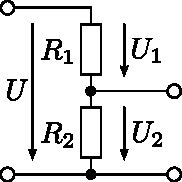
\includegraphics[scale=\schscale]{uteil.pdf}
	\caption{unbelasteter Spannungsteiler}
	\label{sch:uteil}
\end{figure}
\[ U_2 = \frac{U_1}{R_1 + R_2} \cdot R_2 \]

\subsection{belasteter Spannungsteiler}
\begin{figure}[h!]
	\centering
	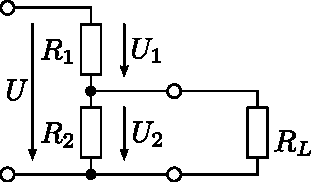
\includegraphics[scale=\schscale]{uteilbel.pdf}
	\caption{belasteter Spannungsteiler}
	\label{sch:uteilbel}
\end{figure}
\[ U_2 = \frac{U_1}{R_1 + \frac{R_2 \cdot R_L}{R_2 + R_L}} \cdot \frac{R_2 \cdot R_L}{R_2 + R_L} \]

\newpage
\subsection{unbelastetes Potentiometer}
\begin{figure}[h!]
	\centering
	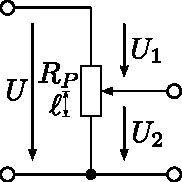
\includegraphics[scale=\schscale]{poti.pdf}
	\caption{unbelastetes Potentiometer}
	\label{sch:poti}
\end{figure}
\[ U_2 = U_1 \cdot \ell \]

\subsection{belastetes Potentiometer}
\begin{figure}[h!]
	\centering
	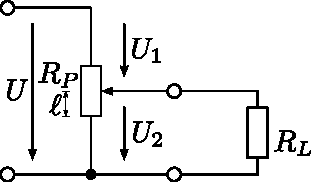
\includegraphics[scale=\schscale]{potibel.pdf}
	\caption{belastetes Potentiometer}
	\label{sch:potibel}
\end{figure}
\[ U_2 = \frac{U_1}{R_p \cdot (1 - \ell) + \frac{R_p \cdot \ell \cdot R_L}{R_p \cdot \ell + R_L}} \cdot \frac{R_p \cdot \ell \cdot R_L}{R_p \cdot \ell + R_L} \]
